\chapter{State of the art analysis}\label{chap:chap3}

This chapter describes the related work associated with this problem, since this area is under explored the following tools are works that follow some analogue methodologies for other project processes like TSP, and some tools that are currently on the market and used for SCAMPI appraisals.

\section{CMMI assessment checklists and tools}
Leaders are recommended to identify the key business capabilities  by conducting a capability maturity assessment \citep{Hutchinson2014}, to determine and find what the organization need to build or strengthen the skills, designed to raise the company, business unit, or specific function to the next level. This tool appear as an online solution to make a lightweight assessment and is a free online assessment that make possible get and track an organization capability across eight key business functions based in a group of 31 questions.


\subsection{Assessment items}
In this tools each assessment item has a statement about a particular capability or several capabilities and a scale that allow to indicate the level of agreement with the statement, based on the organization performance. 

\begin{figure}[h]
	\begin{center}
		\leavevmode
		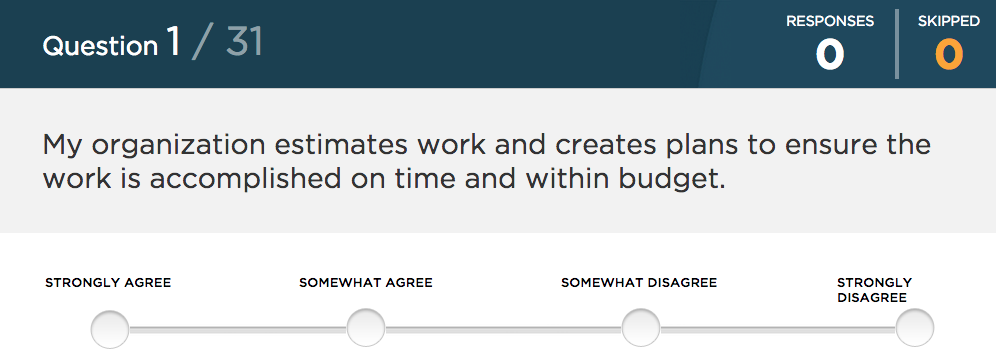
\includegraphics[width=0.75\textwidth]{cmmi_question}
		\caption{Assessment item question}
		\label{fig:cmmi_question}
	\end{center}
\end{figure}

The scale included in the assessment item also includes a descriptive information about the organization performance at both ends of the scale, visible on the example given below.

\begin{figure}[h]
	\begin{center}
		\leavevmode
		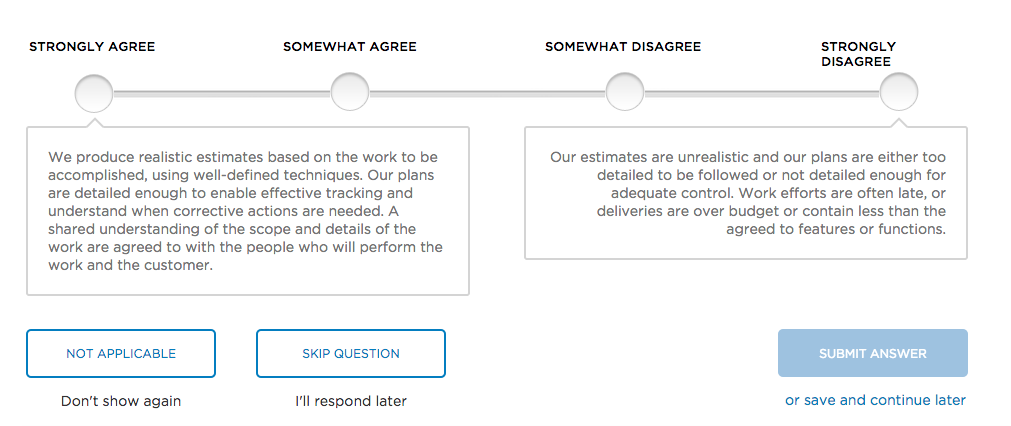
\includegraphics[width=0.86\textwidth]{respostascmmiassessment}
		\caption{Assessment item scale}
		\label{fig:assesment_answer}
	\end{center}
\end{figure}

These descriptions are given to the user with the intention of helping the most accurate positioning of the organization on the scale.

Organization term is defined by the user for purposes of  self-assessment. The evaluated scope is also by the user and can be the company, organizational unit, division, directorate, department or work group.

Its possible to skip a question in the list of items and comeback later to answer and there is an option named Not Applicable to exclude the question from the results, and this answer only should be choose if:
\begin{itemize}
	\item Actual question is related to an area outside of the organization scope.
	\item Its valid for the organization's but the  performance of the activities is not known.
	\item The user that is performing the assessment don't have sufficient expertise in the subject to understand the intent of the question.
\end{itemize}

The answers are editable before the submission of the assessment in a screen for a final review, is possible to save the current state and progress at any time and resume it later. Is only possible to submit and get an assessment if all questions are answered.

After answering all questions provided as requirement and those survey submitted will be show a high level snapshot of the organization  current capability states and will be included in each item some suggestions for developing the next steps.

\begin{figure}[h]
	\begin{center}
		\leavevmode
		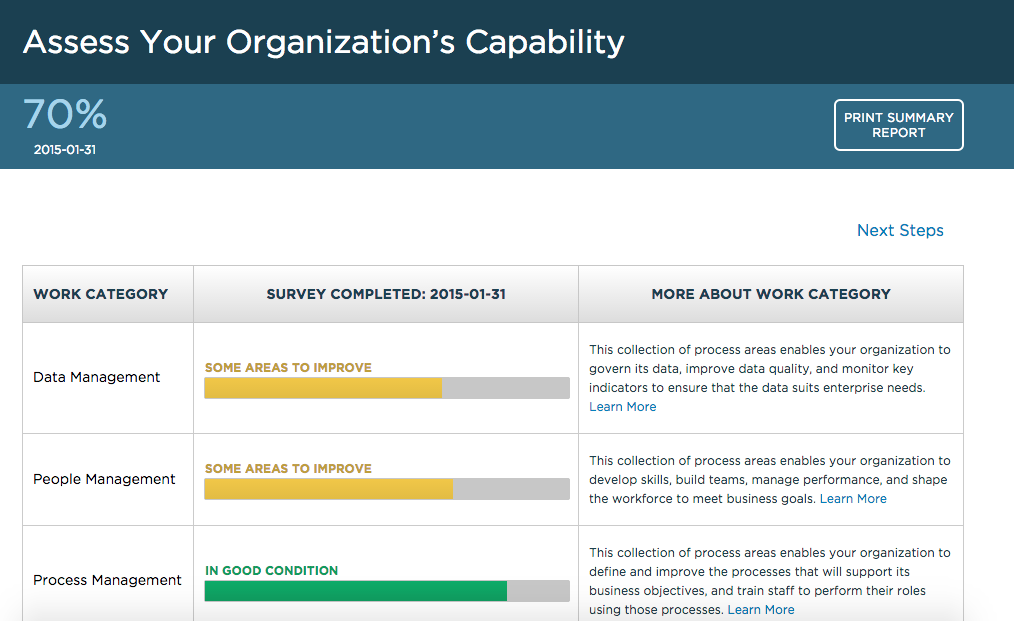
\includegraphics[width=0.96\textwidth]{resultcmmiassessment}
		\caption{Example of a result an assessment}
		\label{fig:assesment_result}
	\end{center}
\end{figure}


\section{PSP/TSP assessment checklists and tools}

PSP\citep{humphrey2005psp} is a process framework with the objective of guide developers to define their own processes, track and plan their work and manage the quality of the produced products.


\subsection{PSPchecker}

PSPChecker\citep{Pinto2010} is a tool that has the main objective of helping teachers to make decisions faster and help students to be able to achieve better results and understand PSP.

Despite PSPChecker was made only for teachers

PSPChecker was planned only to be available to teachers as a support for evaluation and
feedback. But depending on the type of teaching this tool can be also provided to students to improve their work. PSPChecker is user friendly. Users
PSPChecker should provide a simple and intuitive interface that allows users use it after
a short period of learning (Maximum 2 hours). Initially PSPChecker work as a desktop application.

\section{Appraisal and assessment assistant tools}